\documentclass[11pt]{article}
\usepackage{geometry}                % See geometry.pdf to learn the layout options. There are lots.
\geometry{letterpaper}                   % ... or a4paper or a5paper or ... 
%\geometry{landscape}                % Activate for for rotated page geometry
%\usepackage[parfill]{parskip}    % Activate to begin paragraphs with an empty line rather than an indent
\usepackage{graphicx}
\usepackage{amssymb,amsmath}
\usepackage{epstopdf}
\usepackage{pgf}
\usepackage{pgfpages}
\usepackage{tikz}
\usetikzlibrary{arrows,backgrounds}
\usepgflibrary{shapes}
\DeclareGraphicsRule{.tif}{png}{.png}{`convert #1 `dirname #1`/`basename #1 .tif`.png}
\pagestyle{empty}


\begin{document}


 \begin{center}
    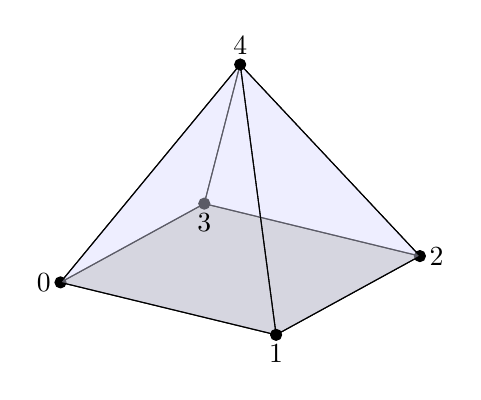
\begin{tikzpicture}[join=round] % pyramid with 5 nodes
       \filldraw[fill=black!20](2.282,.167)--(-.456,.833)--(-2.282,-.167)--(.456,-.833)--cycle;
       \filldraw[fill=blue!10,fill opacity=0.4](0,2.6)--(-2.282,-.167)--(-.456,.833)--(0,2.6)--cycle;
       \filldraw[fill=blue!10,fill opacity=0.4](0,2.6)--(-.456,.833)--(2.282,.167)--(0,2.6)--cycle;
       \filldraw(-.456,.833) circle (2pt);
       \filldraw(2.282,.167) circle (2pt);
       \filldraw[fill=blue!10,fill opacity=0.4](0,2.6)--(2.282,.167)--(.456,-.833)--(0,2.6)--cycle;
       \filldraw(-2.282,-.167) circle (2pt);
       \filldraw[fill=blue!10,fill opacity=0.4](0,2.6)--(.456,-.833)--(-2.282,-.167)--(0,2.6)--cycle;
       \filldraw(0,2.6) circle (2pt);
       \filldraw(.456,-.833) circle (2pt);
       \fill[black]
                (-2.282,-.167) node [left] {0}
                (.456,-.833) node [below] {1}
                (2.282,.167) node [right] {2}
                (-.456,.833) node [below] {3}
                (0,2.6) node [above] {4};
   \end{tikzpicture}
   \hspace{1cm}
   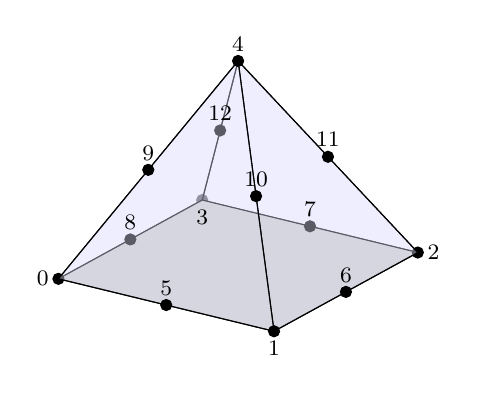
\begin{tikzpicture}[join=round] % pyramid with 13 nodes
        \filldraw(-.456,.833) circle (2pt);
        \filldraw[fill=blue!10,fill opacity=0.4](0,2.6)--(-.456,.833)--(2.282,.167)--(0,2.6)--cycle;
        \filldraw[fill=blue!10,fill opacity=0.4](0,2.6)--(-2.282,-.167)--(-.456,.833)--(0,2.6)--cycle;
        \filldraw[fill=black!20](2.282,.167)--(-.456,.833)--(-2.282,-.167)--(.456,-.833)--cycle;
        \filldraw(.913,.5) circle (2pt);
        \filldraw(-1.369,.333) circle (2pt);
        \filldraw(-.228,1.717) circle (2pt);
        \filldraw(2.282,.167) circle (2pt);
        \filldraw[fill=blue!10,fill opacity=0.4](0,2.6)--(2.282,.167)--(.456,-.833)--(0,2.6)--cycle;
        \filldraw(1.141,1.383) circle (2pt);
        \filldraw(-2.282,-.167) circle (2pt);
        \filldraw[fill=blue!10,fill opacity=0.4](0,2.6)--(.456,-.833)--(-2.282,-.167)--(0,2.6)--cycle;
        \filldraw(-1.141,1.217) circle (2pt);
        \filldraw(1.369,-.333) circle (2pt);
        \filldraw(0,2.6) circle (2pt);
        \filldraw(-.913,-.5) circle (2pt);
        \filldraw(.228,.883) circle (2pt);
        \filldraw(.456,-.833) circle (2pt);
        \fill[black,font=\footnotesize]
                (-2.282,-.167) node [left] {0}
                (.456,-.833) node [below] {1}
                (2.282,.167) node [right] {2}
                (-.456,.833) node [below] {3}
                (0,2.6) node [above] {4}
                (-.913,-.5) node [above] {5}
                (1.369,-.333) node [above] {6}
                (.913,.5) node [above] {7}
                (-1.369,.333) node [above] {8}
                (-1.141,1.217) node [above] {9}
                (.228,.883) node [above] {10}
                (1.141,1.383) node [above] {11}
                (-.228,1.717) node [above] {12};
   \end{tikzpicture}
 \end{center}
 \begin{center}{(a) \hspace{5cm} (b)} \end{center}
 \begin{center}
    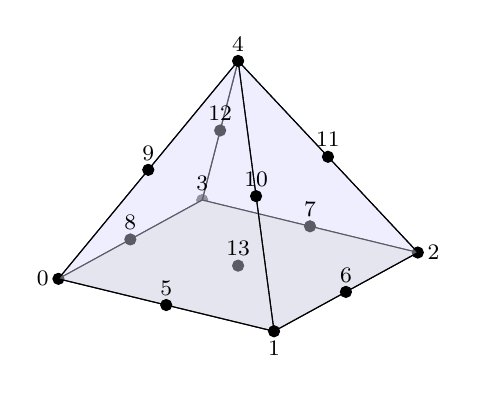
\begin{tikzpicture}[join=round] %pyramid with 14 nodes
         \filldraw(-.456,.833) circle (2pt);
         \filldraw[fill=blue!10,fill opacity=0.4](0,2.6)--(-.456,.833)--(2.282,.167)--(0,2.6)--cycle;
         \filldraw[fill=blue!10,fill opacity=0.4](0,2.6)--(-2.282,-.167)--(-.456,.833)--(0,2.6)--cycle;
         \filldraw[fill=black!10](2.282,.167)--(-.456,.833)--(-2.282,-.167)--(.456,-.833)--cycle;
         \filldraw(.913,.5) circle (2pt);
         \filldraw(-1.369,.333) circle (2pt);
         \filldraw(-.228,1.717) circle (2pt);
         \filldraw(2.282,.167) circle (2pt);
         \filldraw[fill=blue!10,fill opacity=0.4](0,2.6)--(2.282,.167)--(.456,-.833)--(0,2.6)--cycle;
         \filldraw(0,0) circle (2pt);
         \filldraw(1.141,1.383) circle (2pt);
         \filldraw(-2.282,-.167) circle (2pt);
         \filldraw[fill=blue!10,fill opacity=0.4](0,2.6)--(.456,-.833)--(-2.282,-.167)--(0,2.6)--cycle;
         \filldraw(-1.141,1.217) circle (2pt);
         \filldraw(1.369,-.333) circle (2pt);
         \filldraw(0,2.6) circle (2pt);
         \filldraw(-.913,-.5) circle (2pt);
         \filldraw(.228,.883) circle (2pt);
         \filldraw(.456,-.833) circle (2pt);
         \fill[black,font=\footnotesize]
                (-2.282,-.167) node [left] {0}
                (.456,-.833) node [below] {1}
                (2.282,.167) node [right] {2}
                (-.456,.833) node [above] {3}
                (0,2.6) node [above] {4}
                (-.913,-.5) node [above] {5}
                (1.369,-.333) node [above] {6}
                (.913,.5) node [above] {7}
                (-1.369,.333) node [above] {8}
                (-1.141,1.217) node [above] {9}
                (.228,.883) node [above] {10}
                (1.141,1.383) node [above] {11}
                (-.228,1.717) node [above] {12}
                (0,0) node [above] {13};
    \end{tikzpicture}
 \end{center}
 \begin{center}
        (c) 
  \end{center}
\end{document}  
